\chapter{Diseño e implementación} % Main chapter title

\label{Chapter3} % Change X to a consecutive number; for referencing this chapter elsewhere, use \ref{ChapterX}

Este capítulo presenta la solución desarrollada para abordar el análisis multitemporal de la ocurrencia de agua en el Salar de Llullaillaco. Se describen la arquitectura general del sistema, el preprocesamiento aplicado a las imágenes satelitales, el tratamiento de datos climáticos y espectrales, el análisis temporal y la correlación con los indicadores del fenómeno ENSO. Todo el desarrollo ha sido implementado de manera modular, replicable y orientada al uso de plataformas abiertas y datos públicos.


\definecolor{mygreen}{rgb}{0,0.6,0}
\definecolor{mygray}{rgb}{0.5,0.5,0.5}
\definecolor{mymauve}{rgb}{0.58,0,0.82}

%%%%%%%%%%%%%%%%%%%%%%%%%%%%%%%%%%%%%%%%%%%%%%%%%%%%%%%%%%%%%%%%%%%%%%%%%%%%%
% parámetros para configurar el formato del código en los entornos lstlisting
%%%%%%%%%%%%%%%%%%%%%%%%%%%%%%%%%%%%%%%%%%%%%%%%%%%%%%%%%%%%%%%%%%%%%%%%%%%%%
\lstset{ %
  backgroundcolor=\color{white},   % choose the background color; you must add \usepackage{color} or \usepackage{xcolor}
  basicstyle=\footnotesize,        % the size of the fonts that are used for the code
  breakatwhitespace=false,         % sets if automatic breaks should only happen at whitespace
  breaklines=true,                 % sets automatic line breaking
  captionpos=b,                    % sets the caption-position to bottom
  commentstyle=\color{mygreen},    % comment style
  deletekeywords={...},            % if you want to delete keywords from the given language
  %escapeinside={\%*}{*)},          % if you want to add LaTeX within your code
  %extendedchars=true,              % lets you use non-ASCII characters; for 8-bits encodings only, does not work with UTF-8
  %frame=single,	                % adds a frame around the code
  keepspaces=true,                 % keeps spaces in text, useful for keeping indentation of code (possibly needs columns=flexible)
  keywordstyle=\color{blue},       % keyword style
  language=[ANSI]C,                % the language of the code
  %otherkeywords={*,...},           % if you want to add more keywords to the set
  numbers=left,                    % where to put the line-numbers; possible values are (none, left, right)
  numbersep=5pt,                   % how far the line-numbers are from the code
  numberstyle=\tiny\color{mygray}, % the style that is used for the line-numbers
  rulecolor=\color{black},         % if not set, the frame-color may be changed on line-breaks within not-black text (e.g. comments (green here))
  showspaces=false,                % show spaces everywhere adding particular underscores; it overrides 'showstringspaces'
  showstringspaces=false,          % underline spaces within strings only
  showtabs=false,                  % show tabs within strings adding particular underscores
  stepnumber=1,                    % the step between two line-numbers. If it's 1, each line will be numbered
  stringstyle=\color{mymauve},     % string literal style
  tabsize=2,	                   % sets default tabsize to 2 spaces
  title=\lstname,                  % show the filename of files included with \lstinputlisting; also try caption instead of title
  morecomment=[s]{/*}{*/}
}


%----------------------------------------------------------------------------------------
%	SECTION 1
%----------------------------------------------------------------------------------------

\section{Área de estudio y representación espacial}

La cuenca hidrográfica del  Salar de Llullaillaco incluye sectores volcánicos elevados y drenajes que desembocan sobre el salar, esto genera condiciones potenciales para la ocurrencia de cuerpos de agua temporales. Esta delimitación hidrológica se muestra en la figura~\ref{fig:cuenca_llullaillaco}.


\begin{figure}[htpb]
	\centering
	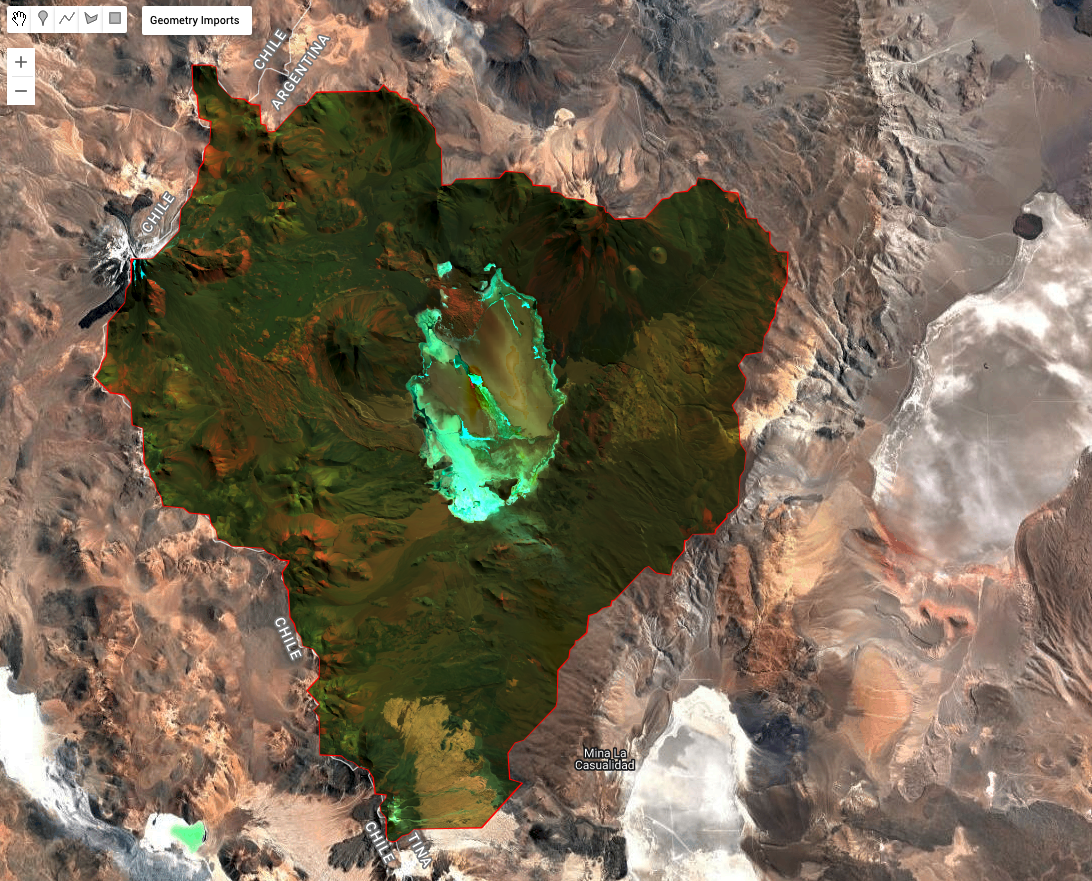
\includegraphics[scale=.3]{Figures/fig5.png}
	\caption{Cuenca del Salar de Llullaillaco.}
	\label{fig:cuenca_llullaillaco}
\end{figure}

Para determinar las zonas con mayor recurrencia de agua superficial, se implementó un procedimiento de clasificación píxel a píxel basado en la aplicación de un umbral de NDWI $>0{,}2$ sobre cada imagen mensual. Este proceso permitió generar una máscara binaria de agua para cada imagen que se integró posteriormente en un mapa de calor de ocurrencia. La proporción de imágenes en las que un píxel fue clasificado como “agua” se interpreta como una probabilidad relativa de presencia hídrica.

El resultado de este análisis se presenta en la figura~\ref{fig:mapa_ocurrencias}, donde se observan claramente las zonas de mayor persistencia de agua dentro del salar.


\begin{figure}[htpb]
	\centering
	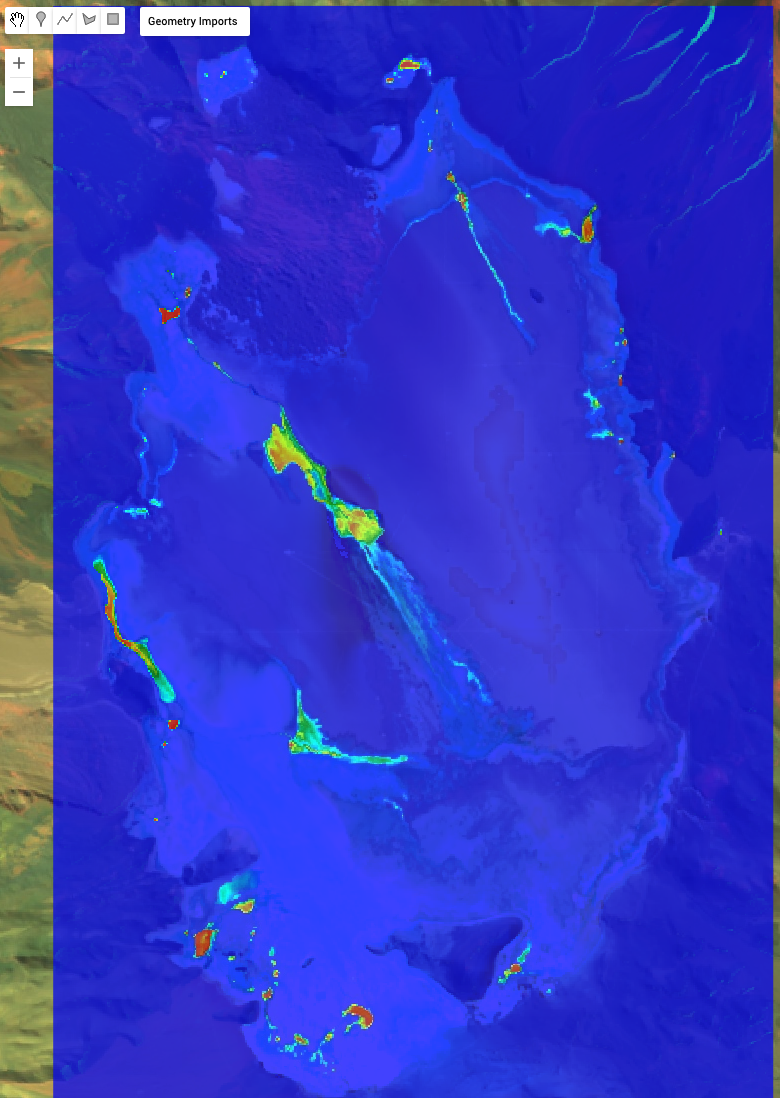
\includegraphics[scale=.3]{Figures/fig6.png}
	\caption{Mapa de calor de ocurrencia de agua superficial en el Salar de Llullaillaco. Colores más cálidos indican mayor frecuencia.}
	\label{fig:mapa_ocurrencias}
\end{figure}



\subsubsection*{Recorte geográfico y generación de mosaicos}

La zona de estudio fue definida a partir de un polígono de delimitación del Salar de Llullaillaco, construido con herramientas SIG y validado mediante visualización satelital. A cada imagen Landsat filtrada se le aplicó un recorte espacial que limita el análisis exclusivamente a esta región.

Dado que cada misión Landsat posee distinto patrón de cobertura espacial, y algunas escenas individuales no cubren completamente el salar, se generaron mosaicos mensuales por misión donde se usó la mediana de los valores de reflectancia en cada píxel. Este procedimiento homogeniza la observación mensual y permite una mejor comparación interanual.


Se observa que la zona con mayor recurrencia de agua corresponde a la laguna central del salar, un cuerpo de agua de morfología alargada, ubicado en el eje norte-sur de la depresión principal. Por este motivo, el análisis estadístico y la posterior implementación de modelos predictivos se enfocan principalmente en esa área. Desde el punto de vista de la biodiversidad esta laguna es la que presenta mayor concentración de fauna acuática.

Las figuras ~\ref{fig:epoca_seca} y ~\ref{fig:epoca_humeda} permiten visualizar el cambio estacional en la extensión de la laguna central del Salar de Llullaillaco, se muestran diferencias notables entre los meses secos y húmedos.


\begin{figure}[ht]
        \centering
        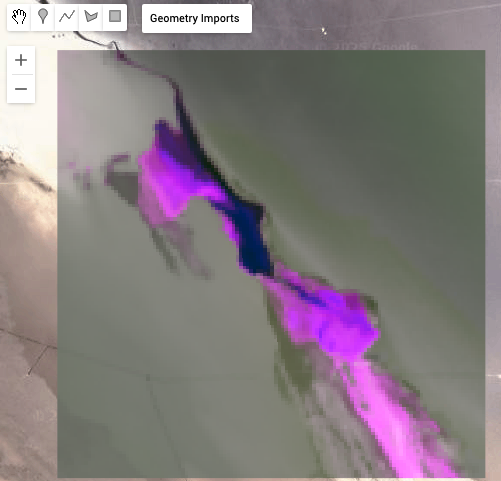
\includegraphics[scale=.37]
        {Figures/fig8_seco.png}
        \caption{Época seca (enero 2015).}
        \label{fig:epoca_seca}
\end{figure}

\begin{figure}[ht]
        \centering
        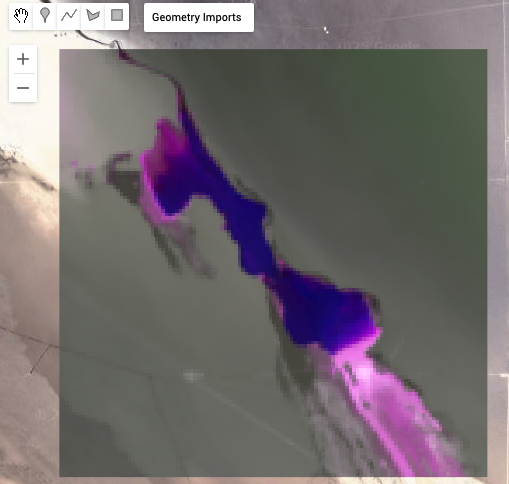
\includegraphics[scale=.37]
        {Figures/fig7_hum.png}
        \caption{Época húmeda (agosto 2021)}
        \label{fig:epoca_humeda}
\end{figure}



Las figuras ~\ref{fig:ndwi_seco} y ~\ref{fig:ndwi_hum}  muestran el resultado del umbral aplicado al índice NDWI para dos fechas representativas. En color verde se observa la clasificación de cuerpos de agua, mientras que el fondo rojo indica ausencia de valores mayores a 0,2. Este umbral ha sido validado en estudios previos para ambientes altoandinos, y permite una segmentación robusta de lagunas frente a suelos secos o salinos.


\begin{figure}[ht]
        \centering
        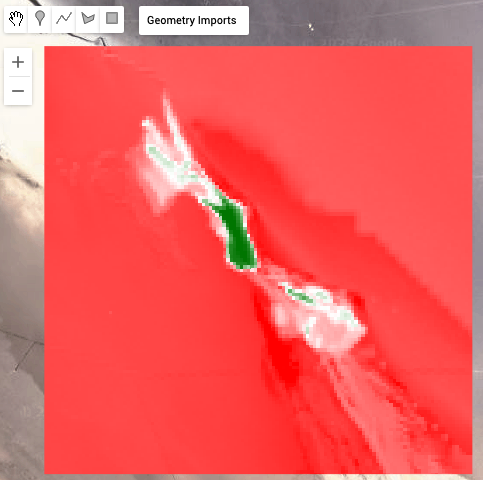
\includegraphics[scale=.37]
        {Figures/fig9_seco.png}
        \caption{NDWI — enero 2015.}
        \label{fig:ndwi_seco}
\end{figure}


\begin{figure}[ht]
        \centering
        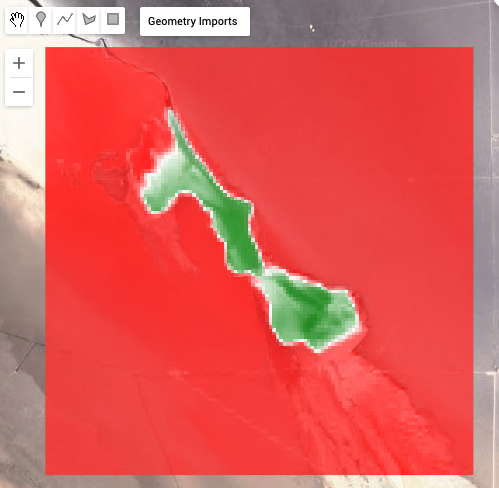
\includegraphics[scale=.37]
        {Figures/fig10_hum.png}
        \caption{NDWI - agosto 2021.}
        \label{fig:ndwi_hum}
\end{figure}

\newpage
\section{Arquitectura general del sistema}

El sistema propuesto se basa en una arquitectura modular que integra tecnologías de teledetección, análisis de datos climáticos y modelado basado en inteligencia artificial. Esta integración permite automatizar el proceso de detección de agua superficial en el Salar de Llullaillaco y explorar su posible relación con variables climáticas globales como las asociadas al fenómeno ENSO.

\subsection*{Componentes principales}

La arquitectura general del sistema se compone de tres bloques funcionales principales (ver figura \ref{fig:arquitectura_general}):

\begin{enumerate}
    \item Bloque de adquisición y preprocesamiento: se encarga de la descarga, filtrado y procesamiento de imágenes satelitales Landsat desde la plataforma GEE. En esta etapa se recorta el área de interés, se eliminan imágenes con cobertura nubosa o mala calidad y se calculan el índices espectral NDWI.
    
    \item Bloque de integración climática: incorpora las series mensuales de los indicadores climáticos ENSO (Niño 3.4, SOI y MEI), obtenidas de fuentes oficiales (NOAA, BOM, PSL), alineadas temporalmente con las imágenes satelitales para permitir su análisis conjunto.

    \item Bloque de análisis y modelado: el análisis incluyó pruebas de estacionariedad (ADF, KPSS, PP), funciones de autocorrelación (ACF, PACF) y la aplicación de modelos SARIMA y VAR, evaluando su capacidad predictiva mediante métricas de error (MSE, RMSE, MAE). Se usaron datos exportados desde GEE y combinados con variables climáticas. La implementación y validación se realizó en Google Colab con Python. De esta manera, se obtuvo replicabilidad, visualización y análisis estadístico de los resultados.
\end{enumerate}

\begin{figure}[htpb]
	\centering
	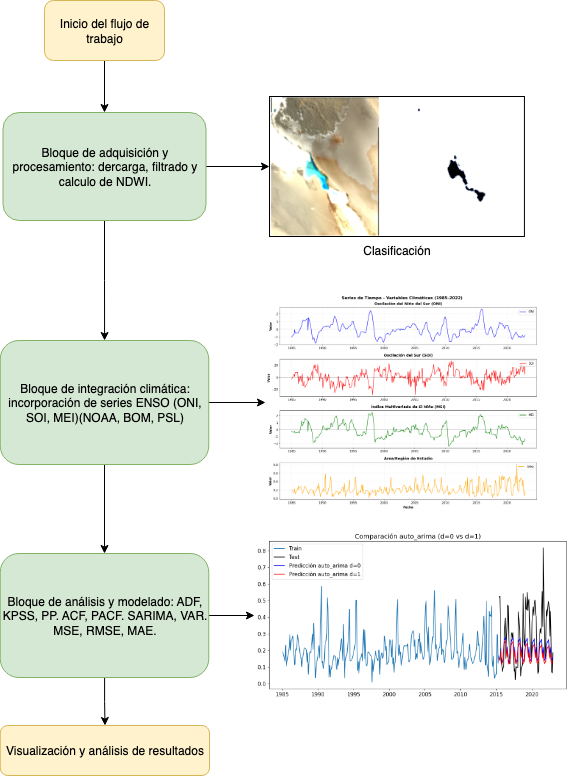
\includegraphics[scale=.6]{Figures/Arqui_TTFB.png}
	\caption{Arquitectura general del sistema: desde la adquisición hasta el modelado.}
	\label{fig:arquitectura_general}
\end{figure}


\subsection*{Flujo de trabajo detallado}

El flujo de trabajo completo incluye las siguientes etapas:

\begin{enumerate}
    \item Extracción satelital: se utilizaron las colecciones \texttt{LANDSAT/LT05/C02/T1\_L2}, \texttt{LANDSAT/LE07/C02/T1\_L2} y \texttt{LANDSAT/LC08/C02/T1\_L2} en GEE. Se seleccionaron imágenes con menos del 20\% de nubosidad y se recortaron al polígono del salar.

    \item Cálculo de índices: se calculó mensualmente los valores medios de NDWI. Se generaron gráficos mensuales y una serie temporal multianual.

    \item Exportación de datos: los datos procesados en GEE fueron exportados en formato CSV y GeoTIFF para su análisis en Python.

    \item Integración con ENSO: se descargaron los valores de Niño 3.4, SOI y MEI, y se alinearon con las fechas de cada imagen mensual. Se realizaron pruebas de normalización y detección de valores atípicos.

    \item Modelado predictivo: se entrenaron modelos exploratorios para predecir la presencia/ausencia de agua en función de los índices espectrales y climáticos. Se utilizaron validaciones cruzadas y análisis de correlaciones.

    \item Visualización de resultados: se generaron mapas de ocurrencia de agua, gráficos de correlación y visualizaciones de precisión de modelos, con el objetivo de interpretar los patrones históricos y su variabilidad.
\end{enumerate}


\subsection*{Ventajas de la arquitectura}

Esta arquitectura ofrece múltiples beneficios:

\begin{itemize}
    \item Permite reproducibilidad total del flujo de trabajo mediante scripts abiertos en GEE y notebooks Python en Colab.
    \item Es escalable a otros salares o humedales de altura, con la modificación del polígono de entrada y el rango de fechas.
    \item Facilita la incorporación de nuevas fuentes climáticas o nuevos sensores remotos sin rediseñar el sistema.
    \item Optimiza el uso de recursos mediante plataformas en la nube, sin requerimientos de hardware local.
\end{itemize}

Esta solución integrada proporciona una herramienta robusta para el análisis ambiental en zonas remotas como la Puna. Su estructura modular, su compatibilidad con datos abiertos y su orientación hacia el análisis multitemporal y predictivo la convierten en una alternativa metodológica replicable en estudios de monitoreo hídrico, cambio climático y gestión territorial.


\section{Preprocesamiento de imágenes}

El preprocesamiento de imágenes satelitales constituye una etapa crítica en todo análisis multitemporal con sensores remotos. En este estudio, se utilizaron imágenes ópticas provenientes de las misiones Landsat 5 TM, Landsat 7 ETM+ y Landsat 8 OLI, accedidas desde la plataforma Google Earth Engine, que permite el procesamiento en la nube con acceso a colecciones históricas de datos corregidos radiométrica y atmosféricamente.

El objetivo del preprocesamiento fue generar series temporales limpias y comparables en el tiempo, con el fin de maximizar la calidad de los datos utilizados para el cálculo de índices espectrales como NDVI y NDWI, los cuales son fundamentales para la detección de cuerpos de agua y vegetación residual. 

\subsubsection*{Selección y filtrado de imágenes}

Las colecciones seleccionadas corresponden a los productos nivel 2 (\texttt{L2}), que contienen valores de reflectancia de superficie corregidos atmosféricamente. Los identificadores de las colecciones utilizadas fueron:

\begin{itemize}
    \item \texttt{LANDSAT/LT05/C02/T1\_L2} para Landsat 5.
    \item \texttt{LANDSAT/LE07/C02/T1\_L2} para Landsat 7.
    \item \texttt{LANDSAT/LC08/C02/T1\_L2} para Landsat 8.
\end{itemize}

El filtrado incluyó:
\begin{itemize}
    \item Eliminación de imágenes con cobertura nubosa mayor al 20\% en la región de interés.
    \item Aplicación de máscaras QA (Quality Assessment) para excluir píxeles cubiertos por nubes, sombras y nieve.
    \item Restricción temporal entre 1990 y 2023, se priorizaron los meses húmedos (enero–abril) para asegurar observaciones relevantes.
\end{itemize}

Este filtrado permitió construir una base de imágenes consistente y sin anomalías atmosféricas notorias, adecuada para los siguientes pasos del análisis.



\subsubsection*{Corrección espectral intersensor}

Debido a diferencias en las respuestas espectrales entre las misiones (especialmente entre TM/ETM+ y OLI), se aplicó una normalización espectral basada en técnicas de remapeo lineal, tal como se propone en la literatura para combinar series temporales Landsat. Esto garantiza que las diferencias observadas en los índices NDWI y NDVI no respondan a variaciones instrumentales sino a cambios reales en superficie.

\subsubsection*{Cálculo de índices espectrales}

Una vez preprocesadas las imágenes, se calcularon los índices espectrales mensuales para cada misión mediante el uso de las bandas adecuadas. Las bandas utilizadas para cada misión se explicaron en capítulos anteriores.

Los valores resultantes fueron exportados como series mensuales promedio para todo el salar, así como también como mapas raster por mes. Esto permitió visualizar la evolución temporal y espacial de la ocurrencia de agua superficial.

\section{Tratamiento de datos }

Esta sección presenta el tratamiento realizado sobre los datos satelitales y climáticos utilizados en el proyecto. Se detallan los criterios de selección, filtrado y preprocesamiento aplicados en la plataforma GEE, así como la integración posterior de variables climáticas globales.

\subsection*{Imágenes satelitales y período de análisis}

Se utilizaron imágenes de las misiones Landsat 5 TM, Landsat 7 ETM+ y Landsat 8 OLI, todas en su versión de corrección atmosférica de superficie (Level 2) disponible en GEE.

El siguiente fragmento de código ilustra la consulta realizada para la colección de Landsat 8:

\begin{verbatim}
var dataset = ee.ImageCollection('LANDSAT/LC08/C02/T1_L2')
  .filterBounds(llullaillaco)
  .filterDate('2015-01-01', '2022-12-31')
  .filterMetadata('CLOUD_COVER', 'less_than', 20)
  .map(applyQAMask)
\end{verbatim}


Si bien la misión Landsat 7 ETM+ estuvo operativa entre 1999 y 2021, su uso en este proyecto fue limitado debido a restricciones de calidad impuestas por el \textit{Scan Line Corrector (SLC)}. Este componente falló en mayo de 2003 desde donde se generaron pérdidas sistemáticas de cobertura espacial en las imágenes posteriores. Aunque en GEE existen funciones para rellenar o enmascarar los bordes afectados, se priorizó evitar la inclusión de imágenes con geometría incompleta o necesidad de interpolación espacial forzada.

La misión Landsat 5 TM fue seleccionada como fuente principal de imágenes anteriores al año 2011, ya que proporcionó datos continuos entre los años 2000 y 2011 sin fallas estructurales. Su cobertura en la región fue consistente durante la ventana húmeda seleccionada (enero a abril), con una densidad de imágenes suficiente para construir una serie temporal representativa.

Por otro lado, Landsat 8 OLI fue utilizado como principal fuente para el período comprendido entre los años 2013 y 2024. 

En la figura ~\ref{fig:cob_temporal} y en la tabla ~\ref{tab:periodos_landsat} se muestran los períodos de tiempo usados. Es necesario mencionar que debido a la superposición entre Landsat 5 TM y Landsat 7 ETM+ se decidió trabajar solo con Landsat 5 TM y Landsat 8 OLI. Se generó un brecha sin imágenes de 12 meses entre febrero de 2012 y febrero de 2013.

\begin{figure}[ht]
        \centering
        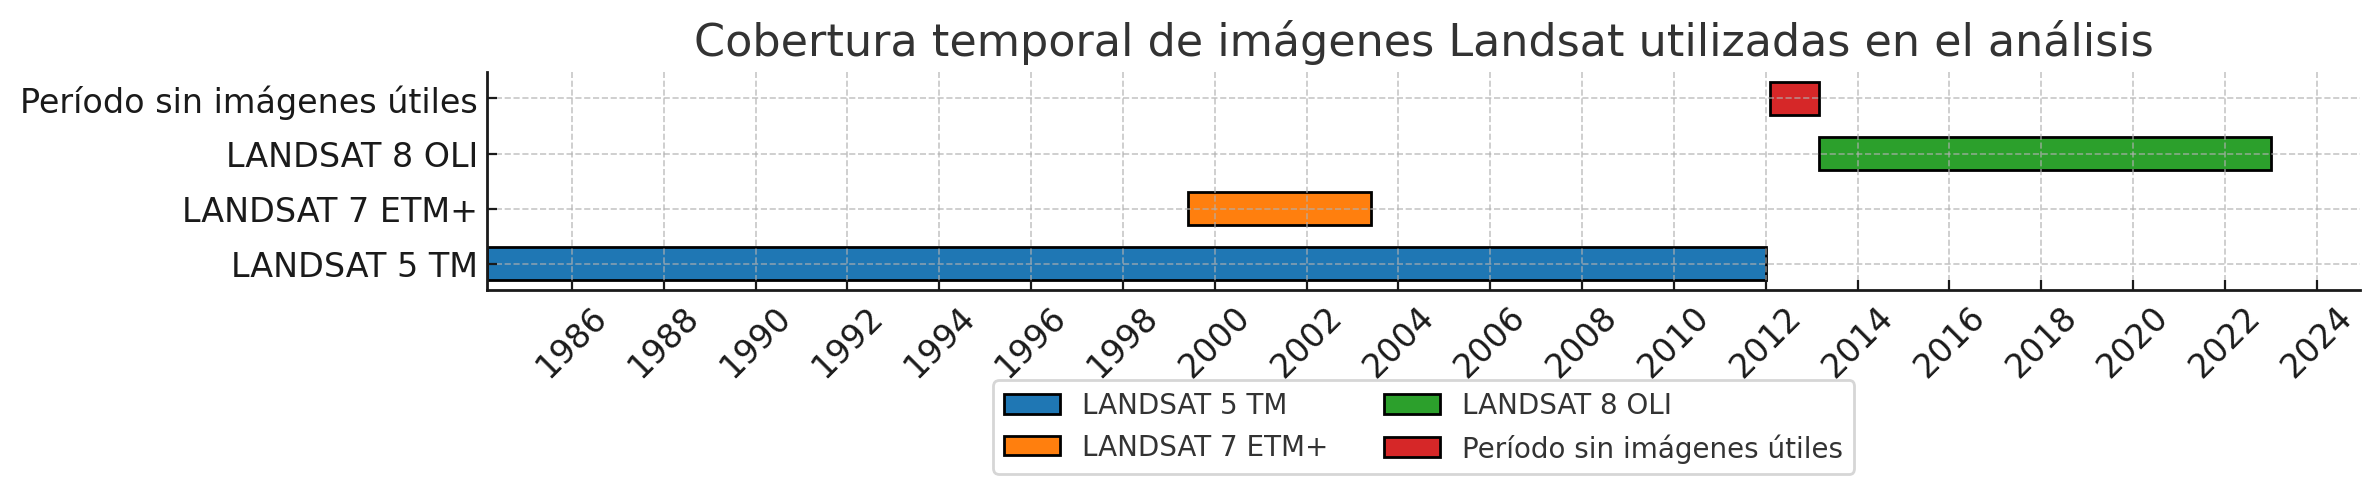
\includegraphics[scale=.4]
        {Figures/fig11.png}
        \caption{Cobertura temporal de las imágenes usadas.}
        \label{fig:cob_temporal}
\end{figure}

En resumen, la elección de misiones respondió a un compromiso entre calidad geométrica, continuidad temporal y cobertura atmosférica, se priorizó la robustez de las series en períodos relevantes para el análisis hidrológico del salar. En la figura ~\ref{fig:cant_imagenes} y en la tabla ~\ref{tab:periodos_landsat} se muestran la cantidad de imagenes usadas. 


\begin{table}[h]
	\centering
	\caption[Períodos Landsat]{Períodos de utilización de imágenes satelitales por misión Landsat en el presente estudio.}
	\begin{tabular}{l c c c}    
		\toprule
		\textbf{Misión}     & \textbf{Inicio (mes/año)} & \textbf{Fin (mes/año)} & \textbf{Cantidad de imágenes} \\
		\midrule
		Landsat 5 TM        & Marzo 1984   & Enero 2012        & 338 \\		
		Landsat 7 ETM+      & Junio 1999   & Mayo 2003         & no se usaran \\
		Landsat 8 OLI       & Marzo 2013   & Diciembre 2022    & 209 \\
		\bottomrule
	\end{tabular}
        \hline
	\label{tab:periodos_landsat}
\end{table}

\begin{figure}[ht]
        \centering
        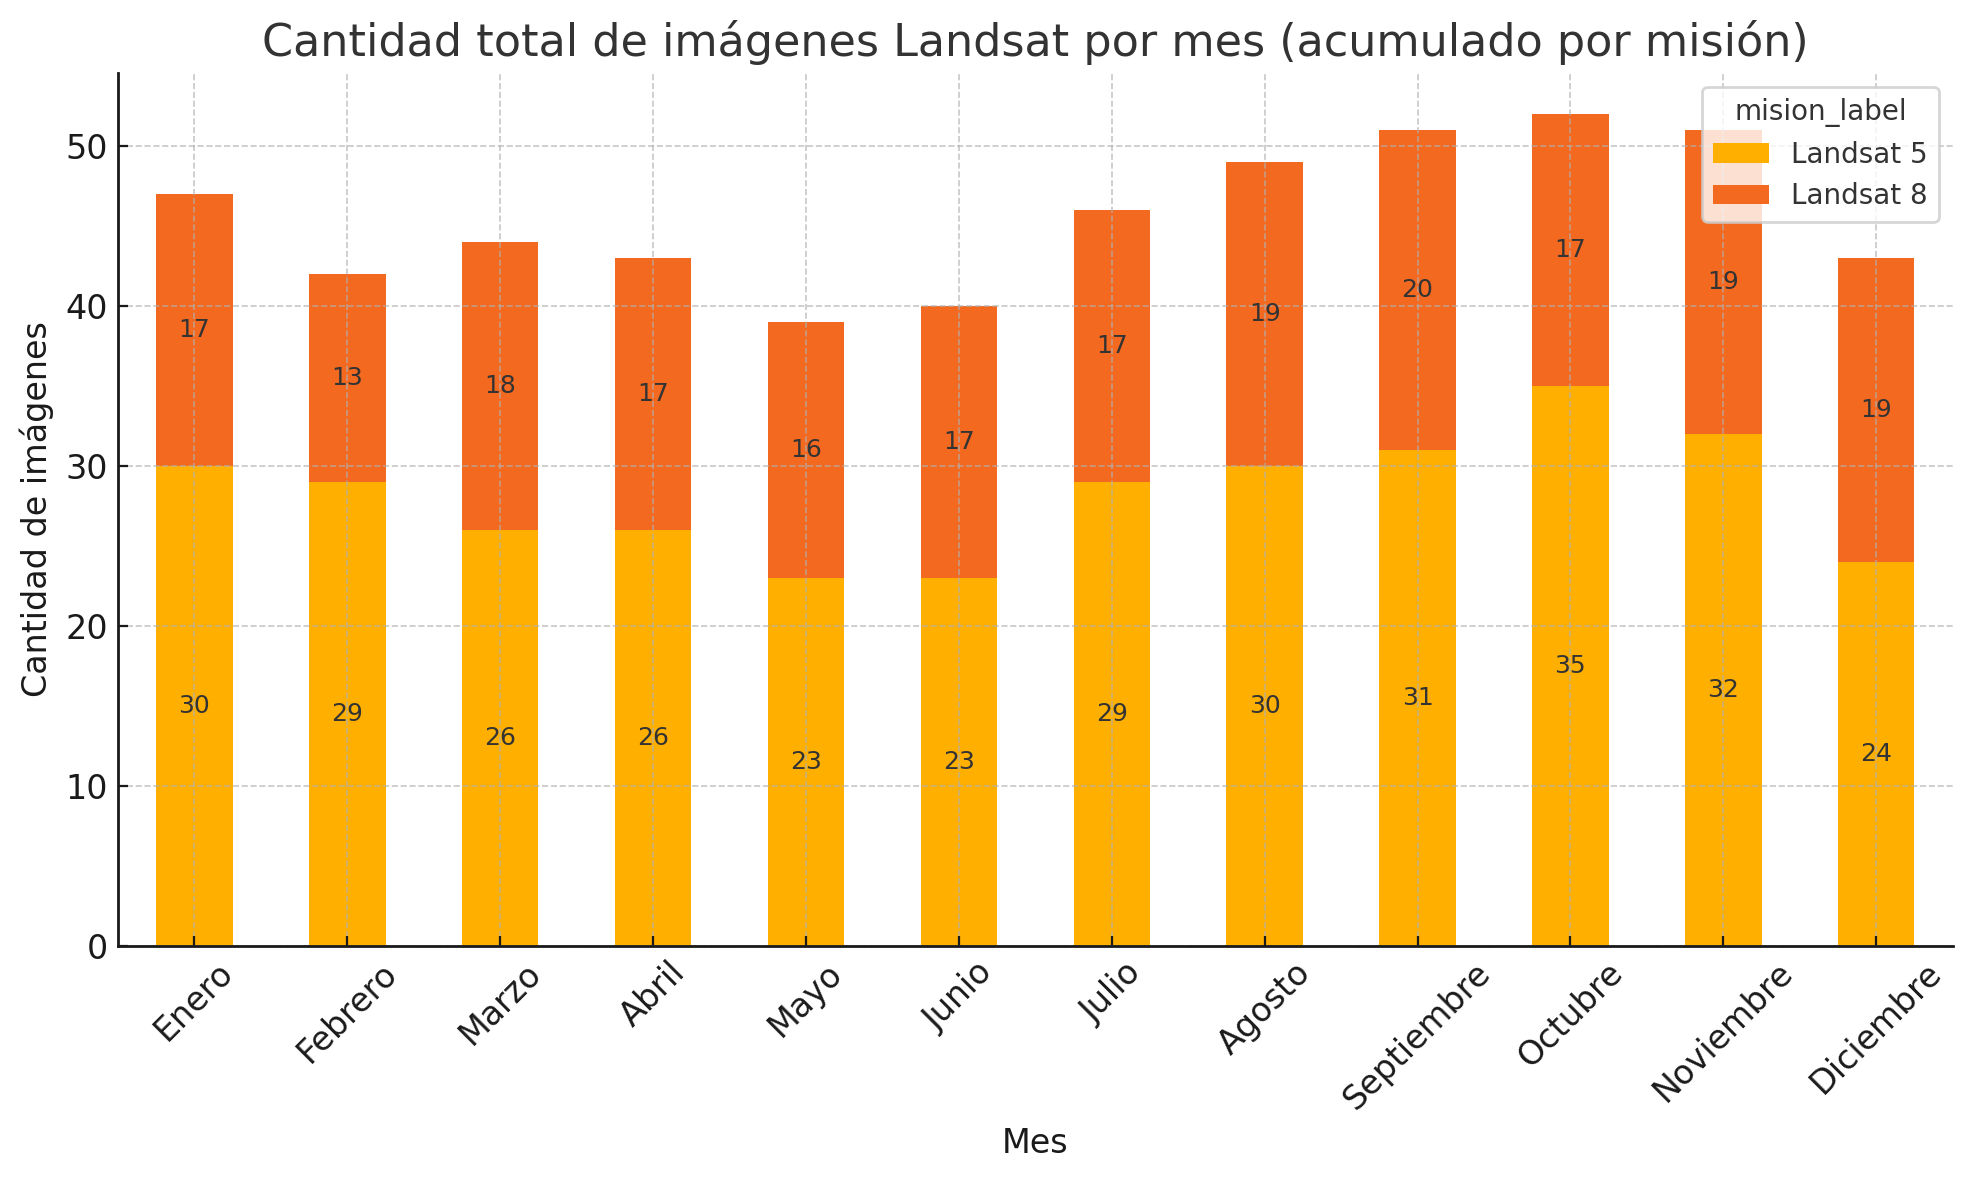
\includegraphics[scale=.4]
        {Figures/fig12.png}
        \caption{Cantidad de imágenes por mes y misión.}
        \label{fig:cant_imagenes}
\end{figure}

\subsection{Datos climáticos globales}

Para integrar la dimensión climática, se descargaron series temporales mensuales de los siguientes indicadores:

\subsubsection{Índice Oceánico de El Niño (ONI)}

El Índice Oceánico de El Niño (ONI, por sus siglas en inglés) es el indicador principal utilizado por la NOAA para monitorear y clasificar los eventos del fenómeno El Niño-Oscilación del Sur (ENSO). Este índice se calcula como la media móvil de tres meses de las anomalías de la temperatura superficial del mar (SST) en la región denominada Niño 3.4, que abarca el área comprendida entre los 5°N–5°S y los 120°W–170°W \citep{noaaONI}.

\textbf{Cálculo del ONI:}
\begin{itemize}
    \item Se basa en las anomalías de SST derivadas del conjunto de datos \textit{Extended Reconstructed Sea Surface Temperature, versión 5 (ERSST.v5)}.
    \item Las anomalías se calculan con respecto a períodos base de 30 años que se actualizan cada cinco años para reflejar los cambios climáticos a largo plazo.
    \item Se emplea una media móvil de tres meses, lo que suaviza las variaciones y permite identificar tendencias sostenidas.
\end{itemize}

\textbf{Clasificación de eventos ENSO según el ONI:}
\begin{itemize}
    \item El Niño: ONI $\geq 0{,}5\,^\circ$C durante al menos cinco períodos consecutivos de tres meses.
    \item La Niña: ONI $\leq -0{,}5\,^\circ$C durante al menos cinco períodos consecutivos de tres meses.
    \item Condición neutral: cuando el ONI se mantiene entre $-0{,}5\,^\circ$C y $0{,}5\,^\circ$C.
\end{itemize}

El ONI es una herramienta ampliamente reconocida y utilizada para identificar eventos ENSO y es considerado una referencia clave para investigaciones climáticas y análisis de correlación entre el océano y patrones hidrometeorológicos continentales. En la figura ~\ref{fig:indice_oni} se muestran los valores de ONI para el período de análisis. 





\subsubsection{Southern Oscillation Index (SOI)}

El índice SOI (\textit{Southern Oscillation Index}) representa la diferencia estandarizada de presión atmosférica a nivel del mar entre Tahití y Darwin, Australia. Este índice captura la componente atmosférica del fenómeno ENSO y es utilizado para caracterizar eventos de El Niño y La Niña desde una perspectiva meteorológica.

Interpretación del índice:

\begin{itemize}
    \item Un SOI positivo (valores mayores a +7) indica presiones relativamente altas en Tahití y bajas en Darwin, condición asociada a La Niña.
    \item Un SOI negativo (valores menores a -7) indica lo contrario, típicamente asociado a El Niño.
    \item Valores entre -7 y +7 se consideran condiciones neutrales.
\end{itemize}

Los valores mensuales y diarios del Índice de Oscilación del Sur (SOI, por sus siglas en inglés) son calculados y publicados por \textit{Australian Bureau of Meteorology}  (BOM) \cite{bom_soi_2024}. En la figura~\ref{fig:indice_soi} se ilustran los valores mensuales del SOI correspondientes al período de análisis.


El SOI se utiliza complementariamente con los índices oceánicos como el ONI, esto permite una caracterización más robusta del fenómeno ENSO desde una perspectiva atmosférica.


\subsubsection{Índice MEI.v2 (\textit{Multivariate ENSO Index versión 2})}

El índice multivariado de El Niño versión 2 (MEI.v2) representa una estimación compuesta del fenómeno ENSO a partir de seis variables atmosféricas y oceánicas observadas en el Pacífico tropical (10°N–10°S, 30°E–70°W). A diferencia de otros índices como el ONI o el SOI, el MEI.v2 utiliza un enfoque multivariado basado en análisis de componentes principales (PCA), lo que permite capturar interacciones complejas entre distintas variables.

Las seis variables utilizadas en su cálculo son: presión al nivel del mar (SLP), temperatura superficial del mar (SST), viento zonal y meridional de superficie (U y V), temperatura del aire en superficie y nebulosidad baja. Estas variables se combinan para derivar una serie normalizada de valores que caracterizan las condiciones del ENSO.

El índice se calcula de manera bimestral móvil, se asocia cada valor a pares de meses consecutivos: Dic-Ene, Ene-Feb, Feb-Mar, y así sucesivamente. Se considera que existe un evento El Niño cuando los valores del índice superan +0{,}5 durante varios bimestres consecutivos, mientras que valores menores a -0{,}5 indican condiciones La Niña. Valores intermedios se interpretan como fase neutral.

Los datos del MEI.v2 se encuentran disponibles desde 1979 hasta la actualidad y son publicados mensualmente por el Physical Sciences Laboratory del NOAA~\cite{meiindex}. Esta serie es empleada en el presente trabajo para evaluar posibles correlaciones climáticas con la presencia de agua en el Salar de Llullaillaco, dentro del período comprendido entre marzo de 1984 y diciembre de 2022. En la figura ~\ref{fig:indice_mei} se muestran los valores de SOI para el período de análisis. 



\section{Series de tiempo preliminares}

Todos los índices climáticos utilizados en este estudio (ONI, SOI y MEI) fueron estandarizados mediante su transformación a \textit{z-score} para facilitar la comparación entre series con distintas escalas y unidades. En la figura~\ref{fig:indice_area} se observa la evolución temporal del área de la laguna de estudio en \textit{z-score}, mientras que en las figuras ~\ref{fig:indice_oni_ts}, ~\ref{fig:indice_soi_ts} y ~\ref{fig:indice_mei_ts} se muestran los índices ONI, SOI y MEI en \textit{z-score} respectivamente.

\begin{figure}[ht]
        \centering
        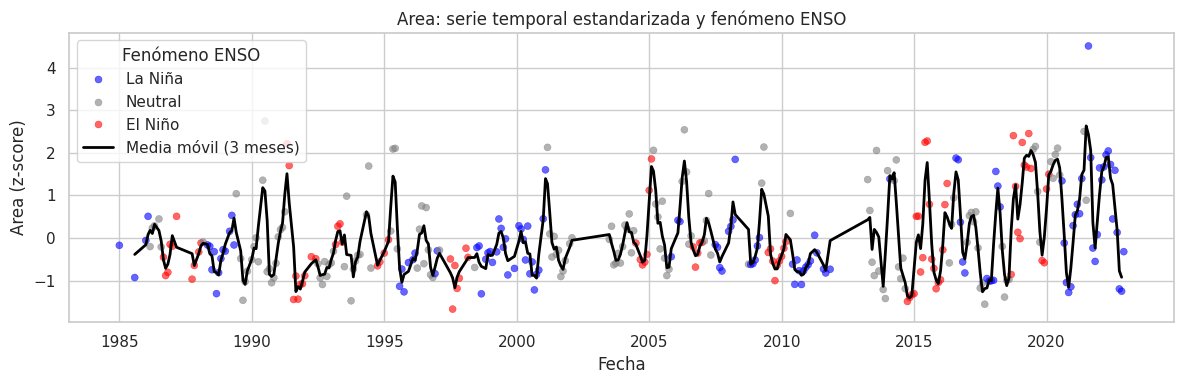
\includegraphics[scale=.45]
        {Figures/fig16_ts_area.png}
        \caption{Área (1984-2022).}
        \label{fig:indice_area}
\end{figure}



Se identificó que las series originales de cobertura de agua superficial y de los índices climáticos ENSO (ONI, SOI y MEI) no eran homogéneas, ya que presentaban vacíos temporales y diferencias en la disponibilidad de datos a lo largo del período de estudio. Esta heterogeneidad impedía su tratamiento directo como series de tiempo y, en consecuencia, limitaba la aplicación de algoritmos de \textit{machine learning} especializados en predicción temporal.  

Por ello, fue necesario realizar un proceso de estandarización y depuración de las series, ajustando su frecuencia y completitud para generar secuencias temporales comparables y aptas para los modelos predictivos. En la Figura~\ref{fig:conteo_datos} se muestra la distribución de meses con datos disponibles por año para cada variable, lo que evidencia la falta de homogeneidad inicial. 

Posteriormente, como se detallará en los capítulos siguientes, se aplicaron técnicas de preprocesamiento y estrategias de imputación para obtener series homogéneas y continuas, que constituyen la base para el análisis de correlaciones y la construcción de modelos predictivos basados en series temporales.  




